\section{Two-dimensional Chiral QFT-I}
\label{sec:2d1}

We have discussed the first-order formalism of topological QM, where the fields are differential forms $\Omega^\blt(S^1,V)$ on $S^1$ valued in the vector bundle $V$ with the de Rham differential $d$. Here $d$ being part of the BRST operator implies that ``translation is homologically trivial.'' This defines a topological theory.

We will now consider 2d chiral models where the fields are complex differential forms, $\Omega^{0,\blt}(\Sigma,h)$ with the Dolbeault differential $\ols{\p}$. The Dolbeault differential being part of the BRST operator implies that ``anti-holomorphic translation is homologically trivial,'' which in turn defines a chiral (or holomorphic) theory.

In topological QM, the theory is \emph{UV finite}, we find that the renormalization process is ``smart'', i.e.
\bea
\begin{tikzcd}
L=0: & ``dI+\hbar\Delta I+\hf\lcb I,I\rcb=0'' 
\ar{d}{e^{\frac{1}{\hbar}I[L]}=\lim_{\varepsilon\to\infty} \exp{(\hbar P^L_\varepsilon)} e^{\frac{1}{\hbar}I}\,\text{exists}} 
&\textit{ill-defined QME}\\
L>0: & dI[L]+\hbar\Delta_L I[L]+\hf\lcb I[L],I[L]\rcb_L=0 
\ar{d}{\text{the (geometrical) meaning of the equation}}[swap]{L\to 0} 
&\textit{well-defined QME}\\
L=0: & dI+\frac{1}{2\hbar} \lsb I,I\rsb=0 
&\textit{local QME}
\end{tikzcd}
\eea
where $[-,-]$ is the Moyal-Weyl commutator. In particular, we find QME = Fedosov equation.
We will see that 2d chiral theory is also \emph{UV finite} and we have a similar geometric result for QME. \textsc{Reference}: \cite{Li:2016gcb}.

\subsection{Vertex algebra}
As discussed in the \nameref{sec:intro}, in 1d topological theory
we have associative algebra defined by the fusion $a\cdot b$; in 2d chiral theory we have (chiral) vertex algebra defined by $A_{(n)}B$. The algebras are found when one operator approaches another either on a line (for 1d) or on a plane (for 2d).
\bea 
\tikzset{every picture/.style={line width=0.75pt}} 
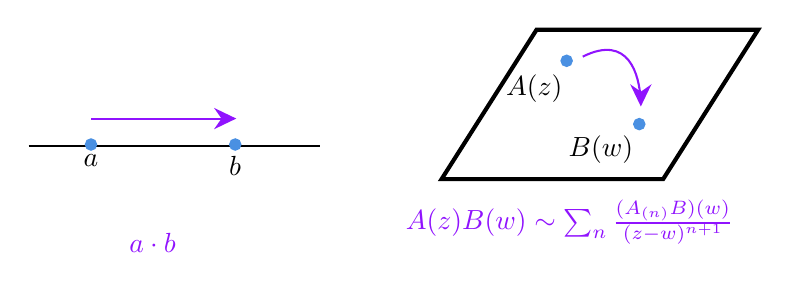
\begin{tikzpicture}[x=0.75pt,y=0.75pt,yscale=-1,xscale=1]

%Straight Lines [id:da21032606992521252] 
\draw    (35.58,72.83) -- (176.08,72.83) ;
%Shape: Circle [id:dp9501490203756839] 
\draw  [color={rgb, 255:red, 74; green, 144; blue, 226 }  ,draw opacity=1 ][fill={rgb, 255:red, 74; green, 144; blue, 226 }  ,fill opacity=1 ] (63.08,72.33) .. controls (63.08,70.95) and (64.2,69.83) .. (65.58,69.83) .. controls (66.96,69.83) and (68.08,70.95) .. (68.08,72.33) .. controls (68.08,73.71) and (66.96,74.83) .. (65.58,74.83) .. controls (64.2,74.83) and (63.08,73.71) .. (63.08,72.33) -- cycle ;
%Shape: Circle [id:dp8390430287126933] 
\draw  [color={rgb, 255:red, 74; green, 144; blue, 226 }  ,draw opacity=1 ][fill={rgb, 255:red, 74; green, 144; blue, 226 }  ,fill opacity=1 ] (132.58,72.33) .. controls (132.58,70.95) and (133.7,69.83) .. (135.08,69.83) .. controls (136.46,69.83) and (137.58,70.95) .. (137.58,72.33) .. controls (137.58,73.71) and (136.46,74.83) .. (135.08,74.83) .. controls (133.7,74.83) and (132.58,73.71) .. (132.58,72.33) -- cycle ;
%Straight Lines [id:da20373559830369148] 
\draw [color={rgb, 255:red, 144; green, 19; blue, 254 }  ,draw opacity=1 ]   (65.75,59.83) -- (132.58,59.83) ;
\draw [shift={(135.58,59.83)}, rotate = 180] [fill={rgb, 255:red, 144; green, 19; blue, 254 }  ,fill opacity=1 ][line width=0.08]  [draw opacity=0] (10.72,-5.15) -- (0,0) -- (10.72,5.15) -- (7.12,0) -- cycle    ;
%Shape: Parallelogram [id:dp8720886994320196] 
\draw  [line width=1.5]  (280.25,17.04) -- (387,17.04) -- (341.25,89) -- (234.5,89) -- cycle ;
%Shape: Circle [id:dp4710229132282462] 
\draw  [color={rgb, 255:red, 74; green, 144; blue, 226 }  ,draw opacity=1 ][fill={rgb, 255:red, 74; green, 144; blue, 226 }  ,fill opacity=1 ] (292.25,32) .. controls (292.25,30.62) and (293.37,29.5) .. (294.75,29.5) .. controls (296.13,29.5) and (297.25,30.62) .. (297.25,32) .. controls (297.25,33.38) and (296.13,34.5) .. (294.75,34.5) .. controls (293.37,34.5) and (292.25,33.38) .. (292.25,32) -- cycle ;
%Shape: Circle [id:dp34299194072766626] 
\draw  [color={rgb, 255:red, 74; green, 144; blue, 226 }  ,draw opacity=1 ][fill={rgb, 255:red, 74; green, 144; blue, 226 }  ,fill opacity=1 ] (327.25,62.5) .. controls (327.25,61.12) and (328.37,60) .. (329.75,60) .. controls (331.13,60) and (332.25,61.12) .. (332.25,62.5) .. controls (332.25,63.88) and (331.13,65) .. (329.75,65) .. controls (328.37,65) and (327.25,63.88) .. (327.25,62.5) -- cycle ;
%Curve Lines [id:da15903818606178466] 
\draw [color={rgb, 255:red, 144; green, 19; blue, 254 }  ,draw opacity=1 ]   (302.5,30) .. controls (324.7,18.9) and (329.79,38.6) .. (330.43,51.12) ;
\draw [shift={(330.5,54)}, rotate = 270] [fill={rgb, 255:red, 144; green, 19; blue, 254 }  ,fill opacity=1 ][line width=0.08]  [draw opacity=0] (10.72,-5.15) -- (0,0) -- (10.72,5.15) -- (7.12,0) -- cycle    ;

% Text Node
\draw (60.58,75.73) node [anchor=north west][inner sep=0.75pt]    {$a$};
% Text Node
\draw (130.58,76.73) node [anchor=north west][inner sep=0.75pt]    {$b$};
% Text Node
\draw (264.08,37.4) node [anchor=north west][inner sep=0.75pt]    {$A( z)$};
% Text Node
\draw (294.25,66.4) node [anchor=north west][inner sep=0.75pt]    {$B( w)$};
% Text Node
\draw (82.58,113.73) node [anchor=north west][inner sep=0.75pt]  [color={rgb, 255:red, 144; green, 19; blue, 254 }  ,opacity=1 ]  {$a\cdot b$};
% Text Node
\draw (215.75,97.4) node [anchor=north west][inner sep=0.75pt]  [color={rgb, 255:red, 144; green, 19; blue, 254 }  ,opacity=1 ]  {$A( z) B( w) \sim \sum _{n}\frac{( A_{( n)} B)( w)}{( z-w)^{n+1}}$};
% Text Node
\draw (359,20.4) node [anchor=north west][inner sep=0.75pt]    {$\bC$};
\end{tikzpicture}
\eea
On a plane, the ``product'' (binary operation) depends on the location holomorphically, leading to $\infty$-ly many binary operations.

\begin{defn}
A \textbf{vertex algebra} is a collection of data:
\begin{itemize}
    \item (space of states) a $\bZ$-graded superspace $\cV=\cV_0\oplus \cV_1$,
    \item (vacuum) a vector $\ket{0}\in \cV_0$,
    \item (translation operator) an even linear map $T: \cV\to\cV$,
    \item (state-field correspondence) an even linear operation (vertex operation) 
    \bea Y(-,z):\cV\to \on{End}\cV[[z,z^{-1}]], \quad A\mapsto Y(A,z)=\sum_{n\in\bZ} A_{(n)}z^{-n-1}\eea
    such that $Y(A,z)B\in \cV((z))$ for any $A,B\in \cV$. 
\end{itemize}
\end{defn}

The data are required to satisfy the following axioms:
\begin{itemize}
    \item (vacuum axiom) $Y(\ket{0},z)=1_{d_\cV}$, i.e. for any $A\in\cV$, 
    \bea Y(A,z)\ket{0}\in \cV[[z]] \quad \text{and} \quad \lim_{z\to0} Y(A,z)\ket{0}=A,\eea
    \item (translation axiom) $T\ket{0}=0$, i.e. for any $A\in\cV$, 
    \bea \lsb T,Y(A,z)\rsb=\p_z Y(A,z),\eea
    \item (locality axiom) all $\lcb Y(A,z)\rcb_{a\in\cV}$ are mutually local.
\end{itemize}

Roughly speaking, mutual locality implies that for any $A,B\in\cV$, we can expand as
\bea Y(A,z)Y(B,w)=\sum_{n\in\bZ}\frac{Y(A_{(n)}\cdot B,w)}{(z-w)^{n+1}}.\eea
This is called the \textbf{operator product expansion (OPE)}. $\lcb A_{(n)}\cdot B\rcb$ from the expansion coefficient can be viewed as defining an infinite tower of products. For simplicity, we will write
\bea A(z)\equiv Y(A,z) \quad \text{for }A\in\cV.\eea
Then the OPE can be written as
\bea A(z)B(w)=\sum_{n\in\bZ}\frac{A_{(n)}\cdot B(w)}{(z-w)^{n+1}}.\eea
We also write, whenever only the \emph{singular} parts matter, 
\bea A(z)B(w)\sim \sum_{n\geq 0}
\frac{A_{(n)}\cdot B(w)}{(z-w)^{n+1}}.\eea

Given a vertex algebra, we can define its \textbf{modes Lie algebra} 
\bea \oint \cV\coloneqq \on{Span}_{\bC}\lcb \oint dz\ z^k A(z)=A_{(k)}\rcb_{A\in\cV,\ k\in\bZ}.\eea
The Lie bracket of contour integrals is determined by the OPE,
\bea \lsb \oint dz\ z^m A(z),\ 
\oint dw\ w^n B(w)\rsb
=\oint dw\ w^n \oint_w dz\ z^m \sum_{j\in\bZ} \frac{A_{(j)}\cdot B(w)}{(z-w)^{j+1}},\eea
where only the singular part matters in the integration. The Lie bracket is represented diagrammatically as follows.
\bea 
\tikzset{every picture/.style={line width=0.75pt}}         
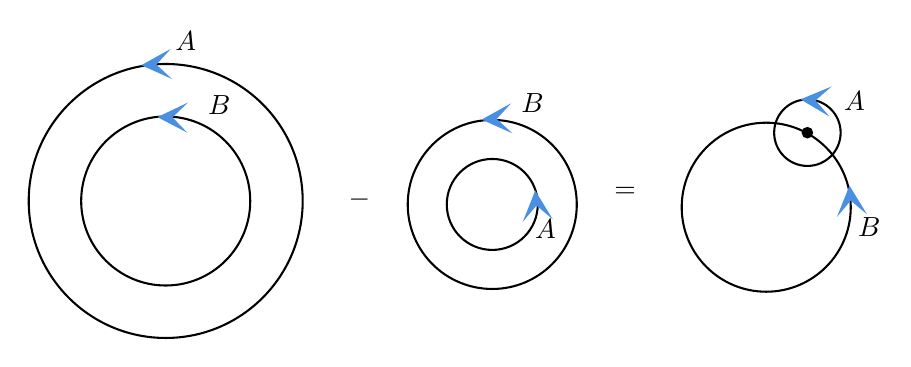
\begin{tikzpicture}[x=0.75pt,y=0.75pt,yscale=-1,xscale=1]


%Shape: Circle [id:dp4986409831322762] 
\draw   (49.33,109) .. controls (49.33,72.55) and (78.88,43) .. (115.33,43) .. controls (151.78,43) and (181.33,72.55) .. (181.33,109) .. controls (181.33,145.45) and (151.78,175) .. (115.33,175) .. controls (78.88,175) and (49.33,145.45) .. (49.33,109) -- cycle ;
%Shape: Circle [id:dp4714377376263692] 
\draw   (74.61,109) .. controls (74.61,86.51) and (92.84,68.28) .. (115.33,68.28) .. controls (137.82,68.28) and (156.06,86.51) .. (156.06,109) .. controls (156.06,131.49) and (137.82,149.72) .. (115.33,149.72) .. controls (92.84,149.72) and (74.61,131.49) .. (74.61,109) -- cycle ;
\draw  [color={rgb, 255:red, 74; green, 144; blue, 226 }  ,draw opacity=1 ][fill={rgb, 255:red, 74; green, 144; blue, 226 }  ,fill opacity=1 ] (115.78,48.51) -- (104.68,43.53) -- (115.32,37.64) -- (110.11,43.3) -- cycle ;
%Shape: Circle [id:dp3866837775378329] 
\draw   (250.75,110.67) .. controls (250.75,98.56) and (260.56,88.75) .. (272.67,88.75) .. controls (284.77,88.75) and (294.58,98.56) .. (294.58,110.67) .. controls (294.58,122.77) and (284.77,132.58) .. (272.67,132.58) .. controls (260.56,132.58) and (250.75,122.77) .. (250.75,110.67) -- cycle ;
%Shape: Circle [id:dp5310956184977278] 
\draw   (231.94,110.67) .. controls (231.94,88.18) and (250.18,69.94) .. (272.67,69.94) .. controls (295.16,69.94) and (313.39,88.18) .. (313.39,110.67) .. controls (313.39,133.16) and (295.16,151.39) .. (272.67,151.39) .. controls (250.18,151.39) and (231.94,133.16) .. (231.94,110.67) -- cycle ;
%Shape: Circle [id:dp15233205654865967] 
\draw   (408.48,76.1) .. controls (408.48,67.25) and (415.65,60.08) .. (424.5,60.08) .. controls (433.34,60.08) and (440.51,67.25) .. (440.51,76.1) .. controls (440.51,84.94) and (433.34,92.11) .. (424.5,92.11) .. controls (415.65,92.11) and (408.48,84.94) .. (408.48,76.1) -- cycle ;
%Shape: Circle [id:dp37578916230390047] 
\draw   (363.94,112) .. controls (363.94,89.51) and (382.18,71.28) .. (404.67,71.28) .. controls (427.16,71.28) and (445.39,89.51) .. (445.39,112) .. controls (445.39,134.49) and (427.16,152.72) .. (404.67,152.72) .. controls (382.18,152.72) and (363.94,134.49) .. (363.94,112) -- cycle ;
%Shape: Circle [id:dp21813935263931072] 
\draw  [fill={rgb, 255:red, 0; green, 0; blue, 0 }  ,fill opacity=1 ] (422.23,76.1) .. controls (422.23,74.84) and (423.24,73.83) .. (424.5,73.83) .. controls (425.75,73.83) and (426.76,74.84) .. (426.76,76.1) .. controls (426.76,77.35) and (425.75,78.36) .. (424.5,78.36) .. controls (423.24,78.36) and (422.23,77.35) .. (422.23,76.1) -- cycle ;
\draw  [color={rgb, 255:red, 74; green, 144; blue, 226 }  ,draw opacity=1 ][fill={rgb, 255:red, 74; green, 144; blue, 226 }  ,fill opacity=1 ] (123.26,74.24) -- (112.47,68.61) -- (123.45,63.36) -- (117.91,68.7) -- cycle ;
\draw  [color={rgb, 255:red, 74; green, 144; blue, 226 }  ,draw opacity=1 ][fill={rgb, 255:red, 74; green, 144; blue, 226 }  ,fill opacity=1 ] (279.78,74.71) -- (268.68,69.73) -- (279.32,63.84) -- (274.11,69.5) -- cycle ;
\draw  [color={rgb, 255:red, 74; green, 144; blue, 226 }  ,draw opacity=1 ][fill={rgb, 255:red, 74; green, 144; blue, 226 }  ,fill opacity=1 ] (432.75,66.32) -- (422.29,60.12) -- (433.53,55.46) -- (427.71,60.5) -- cycle ;
\draw  [color={rgb, 255:red, 74; green, 144; blue, 226 }  ,draw opacity=1 ][fill={rgb, 255:red, 74; green, 144; blue, 226 }  ,fill opacity=1 ] (440.35,113.98) -- (444.86,102.68) -- (451.19,113.07) -- (445.31,108.1) -- cycle ;
\draw  [color={rgb, 255:red, 74; green, 144; blue, 226 }  ,draw opacity=1 ][fill={rgb, 255:red, 74; green, 144; blue, 226 }  ,fill opacity=1 ] (288.95,116.38) -- (293.46,105.08) -- (299.79,115.47) -- (293.91,110.5) -- cycle ;

% Text Node
\draw (118.53,26) node [anchor=north west][inner sep=0.75pt]    {$A$};
% Text Node
\draw (134.27,56.6) node [anchor=north west][inner sep=0.75pt]    {$B$};
% Text Node
\draw (291.87,116.68) node [anchor=north west][inner sep=0.75pt]    {$A$};
% Text Node
\draw (285.2,55.87) node [anchor=north west][inner sep=0.75pt]    {$B$};
% Text Node
\draw (202,102.4) node [anchor=north west][inner sep=0.75pt]    {$-$};
% Text Node
\draw (330,101.07) node [anchor=north west][inner sep=0.75pt]    {$=$};
% Text Node
\draw (440.67,54.73) node [anchor=north west][inner sep=0.75pt]    {$A$};
% Text Node
\draw (447.39,115.4) node [anchor=north west][inner sep=0.75pt]    {$B$};
\end{tikzpicture}
\eea

\begin{eg}[$\beta\gamma$-system]
The $\beta\gamma$-system is generated by two \emph{bosonic} fields $\beta(z), \gamma(z)$ with the contractions
\bea \beta(z)\gamma(w)\sim \frac{\hbar}{z-w}\sim -\gamma(z)\beta(w).\eea
The vertex algebra $\cV$ is identified with the differential ring
\bea\cV= \nord{\bC[[\p^i\beta,\p^i\gamma]]} [[\hbar]],\eea
where $\nord{\ }$ is the \emph{normal ordering operator}. The general OPE is obtained via \textbf{Wick contractions}. For example,
\bea \nord{\beta(z)\gamma(z)} \nord{\beta(w)\gamma(w)}
&= \underbrace{\frac{\hbar}{z-w} \nord{\gamma(z)\beta(w)}- 
\frac{\hbar}{z-w} \nord{\beta(z)\gamma(w)}}_{\text{1 contraction}}
-\underbrace{\lb\frac{\hbar}{z-w}\rb^2}_{\text{2 contractions}}\\
&=\sum_{k\geq 0}\frac{\hbar}{z-w}\frac{(z-w)^k}{k!} \nord{\p^k\gamma(w)\beta(w)-\p^k\beta(w)\gamma(w)} -\frac{\hbar^2}{(z-w)^2}.\eea
\end{eg}

\begin{eg}[$bc$-system]
The $bc$-system is generated by two \emph{fermionic} fields $b(z), c(z)$ with
\bea b(z)c(w)\sim \frac{\hbar}{z-w}\sim c(z)b(w).\eea
The vertex algebra $\cV$ is identified with the differential ring
\bea\cV= \nord{\bC[[\p^i b,\p^i c]]} [[\hbar]].\eea
The general OPE is generated in the similar way as the $\beta\gamma$-system (but we need to take care of the signs). 
\end{eg}

More generally, we can define a general $\beta\gamma-bc$ system by considering a $\bZ_2$-graded space 
\bea h=h_0\oplus h_1\eea 
with an even symplectic pairing
\bea \lan -,-\ran: \asym^2 h\to \bC.\eea
Let $\lcb a_i\rcb$ be a basis of $h$, then we can define a vertex algebra $\cV_h$ by
\bea\cV_h= \nord{\bC[[\p^k a_i]]} [[\hbar]].\eea
The OPE is generated by
\bea a_i(z)a_j(w)\sim \frac{\hbar}{z-w} \lan a_i,a_j\ran.\eea
In particular, $h_0$ represents the copies of $\beta\gamma$-system; $h_1$ represents the copies of $bc$-system. 

\subsection{Chiral deformation of $\beta\gamma-bc$ systems}
We consider the following data:
\begin{itemize}
    \item an elliptic curve $E$ (topologically a torus $T^2$) with linear coordinate $z$ such that $z\sim z+1\sim z+\tau$,
    \item a graded symplectic space $h=h_0\oplus h_1$ with an even symplectic pairing $\lan -,-\ran$.
\end{itemize}
This defines a field theory in BV formalism by
\bea \begin{cases} \text{fields}:\ \cE=\Omega^{0,\blt}(E)\otimes h,\\
(-1)-\text{symplectic pair}: \omega(\varphi_1,\varphi_2)=\int_E dz\wedge \lan \varphi_1,\varphi_2\ran, \quad \varphi_i\in\cE. \end{cases}\eea
Note that $\omega$ has $\on{deg}=-1$ since we need exactly one $\ols{dz}$ from $\varphi_1,\varphi_2$ to be integrated.

The free theory is given by 
\bea \hf\int_E dz\lan \varphi
,\pb \varphi\ran, \quad \varphi\in\cE.\eea
The local quantum observables form exactly $\beta\gamma-bc$ system. Th propagator is given by \textbf{Szeg\H{o} kernel}
\bea \pb^{-1}\sim \frac{1}{z-w}+\text{regular}.\eea
We would like to consider a general interacting theory by turning on \textbf{chiral deformations}, such that we have
\bea \int \cL\lb \varphi,\p_z\varphi,\p_z^2\varphi,\cdots\rb\eea
which involves only \emph{holomorphic} derivatives. This is related precisely to the vertex algebra
\bea \cV_{h^\vee}= \bC[[\p^i h^\vee]] [[\hbar]]\eea
as follows. Define a map
\bea I: \cV_{h^\vee}\to \sO_{loc}(\cE), \quad \gamma\mapsto I_\gamma.\eea
Explicitly, if $\gamma=\sum \p^{k_1}a_1\cdots \p^{k_m}a_m$, then \bea I_\gamma(\varphi)=i\int_E dz \sum\pm \p^{k_1}_z a_1(\varphi)
\p^{k_m}_z a_m(\varphi).\eea
Here $a_i\in h^\vee$ and $a_i(\varphi)\in \omega^{0,\blt}(E)$.

\begin{thm}[UV finiteness]
For any $\gamma\in \cV_{h^\vee}$, the chiral deformed theory
\bea \hf \int_E dz\lan \varphi,\pb \varphi\ran +I_\gamma(\varphi)\eea
is \textbf{UV finite} in the sense that
\bea e^{\frac{1}{\hbar}I_\gamma[L]}=\lim_{\varepsilon\to 0} \exp{(\hbar P^L_\varepsilon)} e^{\frac{1}{\hbar}I_\gamma}\eea
exists.
\end{thm}

\begin{rmk}
The proof to the UV finiteness theorem is a bit technical. Interested reader may refer to \cite{Li:2016gcb}. The reason is different from topological QM, where we saw that the propagator is bounded (although not continuous). Here the graph integral is NOT absolute convergent. See the next section for a geometric interpretation of this fact.
\end{rmk}

Once we have a well-defined $I_\gamma[L]$ described above, we can formulate the \textbf{effective QME}
\bea \pb I_\gamma[L]+\hbar\Delta_L I_\gamma[L]+\hf\lcb I_\gamma[L],I_\gamma[L]\rcb_L=0\eea
and ask for the condition of $\gamma$ to satisfy the equation. It turns out that the answer is very simple.

\begin{thm}[Li \cite{Li:2016gcb}]
Consider $\gamma\in \cV_{h^\vee}$ and the effective functional $I_\gamma[L]$ defined above via the UV finiteness. Then $I_\gamma[L]$ satisfies the effective QME
\bea \pb I_\gamma[L]+\hbar\Delta_L I_\gamma[L]+\hf\lcb I_\gamma[L],I_\gamma[L]\rcb_L=0\eea
if and only if 
\bea \lsb \oint\gamma,\oint\gamma\rsb=0 \ \in \oint \cV.\eea
\end{thm}

\begin{rmk}
The local quantum observable of the chiral deformed theory is the vertex algebra $H^\blt(\cV_{h^\vee},\oint \gamma)$. So $\oint \gamma$ plays the role of BRST reduction. Reversely, vertex algebras coming from the BRST reduction of free field realizations can be realized via the model of chiral deformations above.
\end{rmk}

The above theorem can be glued for a \emph{chiral $\sigma$-model}
\bea \varphi:E\to X\eea
which produces a bundle $\cV(X)\to X$ of chiral vertex algebras on $X$. Then the solution of effective QME asks for a flat connection on $\cV(X)$ of the form
\bea D=d+\frac{1}{\hbar}\lsb \oint\gamma,-\rsb, \ \text{such that}\ D^2=0.\eea
Here $\gamma\in\Omega^1\lb X,\cV(X)\rb$ and $\oint \gamma$ is fiberwise chiral mode operator. This can be viewed as the \emph{chiral analogue of Fedosov connection}.
